\documentclass[thesis.tex]{subfiles}
\begin{document}
All this theory allows us to actually implement the estimator, and present some (interesting) results.
With this implementation we will analyze the unknown constants still present in the error bounds. 
In particular, how tight is the error bound given by the equilibrated residual estimator?
What is the practical convergence rate of AFEM driven by the equilibrated estimator?
How do the equilibrated and classical estimator --- both optimal AFEM drivers --- compare to eachother?


  MATLAB \cite{MATLAB:2015} will be used for the actual implementation. We also
  make extensive use of iFEM \cite{chenifem}, a general framework for adaptive finite element methods. 
  We let iFEM framework  calculate a \emph{linear} discrete solution $U_h$ for a given partition.
  The package ships with an implementation of the \emph{newest vertex bisection} refinement algorithm.\todo{Do
  we need to introduce this anywhere else?} This refinement method bisects triangles and ensures conformity of the resulting triangulation,
  and in addition ensures that the produced triangulation is shape regular with respect to the initial triangulation.
  We will first asses some (normal) finite element solutions.  After this we will
  consider the performance of AFEM driven by the (first order) equilibrated estimator. The results
  will be compared to the classical residual estimator.

  \section{Exact error}

  For meaningful results we ideally compare our error bounds to the \emph{exact} error $\enorm{u - U_h}_\O$. Unfortunately this is
  not possible is most situations. If one knows the exact solution $u$ of an interesting problem, then
  the right hand side $f$ of the associated Poisson problem is almost never constant, rendering our implementation useless. 
  We have two ways to overcome this problem. 
  
  The first is to treat the $f$ as if it was piecewise constant; that is, 
  we approximate $\ip{\psi_a f - \nabla \psi_a \nabla U_h, q_k}_K$ by the edge-midpoint quadrature and ignore this approximation error. Similarly we simply replace $\uanorm{f - \div \v{\zeta}}_K$ \todo{this upper bound is not introducd} by its edge-midpoint quadrature. Provided that $f$ is sufficiently smooth, the effects of these extra errors are of higher order $h$, and thus should wary of for small diameter.
  
  The other approach is using a constant $f$, without knowing the exact solution $u$. We propose to approximate the true error $\enorm{u - U_h}_\O$ by replacing $u$ with another finite element solution $\tilde U_h$  --- quite dazzling if one thinks about it.
  To make this work we let $\tilde U_h$ be a solution on a finer triangulation $\tilde \T_h \geq \T_h$, such that
  every element in $\tilde \T_h$ is at least \emph{one} bisections away from its corresponding element in $\T_h$. We have
  \[
    \enorm{u - U_h}_\O \leq \uaenorm{u - \tilde U_h}_{\O} + \uaenorm{U_h - \tilde U_h}_{\O},
  \]
  where we hope --- which is most likely the case if $u$ possesses some smoothness --- that $\uanorm{u - \tilde U_h}_{\O} \ll \uanorm{U_h - \tilde U_h}_{\O}$. The straightforward implementation follows from noting that $U_h$ is also in the finite element spaces of refine triangulations.  iFEM  conviently provides a function that calculates the coefficients of $U_h$ with respect to the linear basis on a refined triangulation.
  \todo{impl iFEM}
  \section{Unit square}
  Take $\O = (0,1)\times(0,1)$ with exact solution $u(x,y) = \sin(2\pi x)\sin(2\pi y)$, and thus
  \begin{equation}
    \label{eq:squaresin}
    \begin{alignedat}{2}
      -\Delta u &= 8\pi^2\sin(2\pi x)\sin(2\pi y)  \quad &&\text {in } \Omega, \\
      u &= 0 \quad &&\text{on } \partial\O.
    \end{alignedat}
  \end{equation}
  The exact solution has four peaks and is very smooth. We let iFEM calculate the discrete solutions $(U_k)_{k \geq 0}$ for 
  a sequence of uniformly bisected triangulations, i.e. every triangle is bisected into four subtriangles. It uses third order quadrature to approximate the integrals containing $f$. The produced result is illustrated in Figure~\ref{fig:squareuh}.

  \begin{figure}
    \centering
        \includegraphics[width=.32\linewidth]{mesh_square_1.png}
        \includegraphics[width=.32\linewidth]{mesh_square_3.png}
        \includegraphics[width=.32\linewidth]{square_result_8.png}
        \caption{The finite element solutions $U_k$ for \eqref{eq:squaresin} with  uniformly bisected triangulations, from left to right we have diameters $h = 2^{-1}, 2^{-3}, 2^{-8}$.}
    \label{fig:squareuh}
\end{figure}
The images clearly indicate convergence of the FEM solution. 
As $u \in H^2(\O)$ we expect that $\enorm{u - U_k}_{\O} \lesssim h \abs{u}_{H^1(\O)}$. For uniform refinements this
latter is equivalent to $\enorm{u - U_k}_{\O} \lesssim N^{1/2} \abs{u}_{H^1(\O)}$, with $N$ the total number of vertices.

The iFEM package provides a method to calculate $\enorm{u - U_h}_{\O}$ given the exact $u$, 
and also provides an implementation of the standard residual estimator $\hat \eta_\T(U_h, \T)$.
We compare these against the equilibrated upper bound from \eqref{eq:zetaupper},  i.e.
\[
  \enorm{u - U_h}_{\O} \leq \sqrt{\sum_{K \in \T_h} \left[ \uanorm{\vzet + \nabla U_h}_{K} + \frac{h_K}{\pi} \uanorm{ f - \div\v{\zeta}}_{K}\right]^2}.
\]
We also calculate their efficiency indices as $\enorm{u - U_k} / \eta$. In the equilibrated case we would like this value to be close to one, as this shows tightness of the estimator. In the residual case we have an extra constant in the reliability bound, and thus tightness depends also depends on this (unknown) constant.
The results are given in Figure~\ref{fig:squareerror}. The experimental convergence rate is in line with the theoretical convergence rate.
\begin{figure}
  \centering
  \includegraphics[width=.49\linewidth]{squaresin_norm_slope_9.eps}
  \includegraphics[width=.49\linewidth]{squaresin_efficiency_9.eps}
  \caption{The left compares the exact error in the energy norm with the standard residual estimator, and the equilibrated residual estimator.
    These are calculated for discrete solutions $U_k$ of \eqref{eq:squaresin} for a sequence of uniformly refined triangulations. 
    The triangle has a slope of $-1/2$.  
  The right figure plots $\enorm{u - U_k} / \eta$; an estimation of the efficiency index.}
  \label{fig:squareerror}
\end{figure}

Even though we calculated the equilibrated estimator for $p=0$, it still proves to be real close to the actual error. The efficiency index
seems to increase, which could be explained by a reduction  in the influence of quadrature errors for smaller diameters. We have the exact solution
$u$ for this system, and thus we can empirically verify the claim that $\enorm{u - U_k}_{\O}$ is more or less equal to $\enorm{U_{k+i} - U_k}_{\O}$ for $i\geq 1$. The results for this problem with $i=1,2,3$ are given in Figure~\ref{fig:squareapprox}. The quality
of the error approximation increases with $i$ as expected. 
\begin{figure}
  \centering
  \includegraphics[width=.49\linewidth]{squaresin_approx_H1_10.eps}
  \includegraphics[width=.49\linewidth]{squaresin_approx_H1_rel_10.eps}
  \caption{ The exact error $\enorm{u - U_k}_{\O}$ is compared to the approximation $\enorm{U_{k+i} - U_k}_{\O}$ for $i=1,2,3$. The
    left image all of these terms are separately visualised, which results in a cluttered image as expected. The right image
  displays the relative terms, i.e. $\enorm{U_{k+i} - U_k}_{\O} / \enorm{u - U_k}_{\O}$.}
  \label{fig:squareapprox}
\end{figure}


Another Poisson problem for the unit square domain is given by 
\[
  u(x,y) = 2^{40}x^{10}(1-x)^{10}y^{10}(1-y)^{10}.
\]
The corresponding right hand side $f$ is a high order polynomial; we let Matlab derivate  it using symbolic calculations. The
solution $u$ has a peak of value $1$ centered around $(\frac{1}{2}, \frac{1}{2})$ and is again very smooth. In Figure~\ref{fig:squareana}
the efficiency indices are given, alongside the relative errors generated by $\enorm{U_{k+i} - U_k}_{\O}$ for this new problem. The 
initial triangulation $\T_0$ is equal the one used in the previous problem.
The efficiency of the equilibrated estimator is less for this problem, which is most likely due to the large oscillation factor,
but it still outperforms the classical residual estimator. 

The behaviour of $\enorm{U_{k+i} - U_k}_\O$ is very similar to that of the previous problem, it appears to be a good estimation of $\enorm{u - U_k}_{\O}$. We will therefore use this in the following problems, due to the absence of an exact solution. 
For accuracy reasons we pick $i=3$, which should be enough for a `true error' indication.
We will write $\wt U_k$ for the discrete solution found on the three time uniformly refined triangulation of $\T_k$.

\begin{figure}
  \centering
  \includegraphics[width=.49\linewidth]{squareana_efficiency_9.eps}
  \includegraphics[width=.49\linewidth]{squareana_approx_H1_rel_10.eps}
  \caption{Left image compares the efficiency indices of the standard residual estimator with the equilibrated estimator. Right image
  shows the exact error approximation quality.}
  \label{fig:squareana}
\end{figure}

\section{Re-entrant corner}
Here $\O = (-1,1)^2\setminus[-1,0]^2$ with right hand side $f = \1$; this is also known as the L-shaped domain. 
The solution $u$ of this problem has a singularity at the origin so
that $u \not \in H^2(\O)$. The theoretical
convergence on uniform refined triangulations is of order $h^{2/3}$. We calculate  discrete solutions $U_k$ for uniform refinements, and use $\uaenorm{\wt U_k - U_k}_\O$ to approximate the true error. 

The results are given in Figure~\ref{fig:lshapeone}. The experimental
convergence of the fem solution appears to match the theoretical convergence. 
The equilibrated residual once again has a better efficiency index than the residual estimator.
There is a drop in terms of efficiency compared to the previous problems. Interestingly, the efficiency of the equilibrated
estimator seems to decrease, whereas the efficiency of the standard estimator is somewhat increasing. 
This might be related to the approximation quality of $\enorm{\tilde U_k - U_k}_{\O}$.

\begin{figure}
  \centering
  \includegraphics[width=.49\linewidth]{lshapeone_norm_8.eps}
  \includegraphics[width=.49\linewidth]{lshapeone_efficiency_8.eps}
  \caption{Error estimators and their efficiency for the re-entrant corner problem. The triangle has a slope of $-1/3$.}
  \label{fig:lshapeone}
\end{figure}

\section{Crack domain}
A problem with a line singularity is given by the crack domain: take $f = \1$ and
\[
  \O=\{(x,y) \in \R^2 : |x|+|y|<1\}\setminus ([0,1] \times \set{0}).
\]
The exact solution $u$ can be given in polar coordinates, $u(r, \phi) = r^{1/2}\sin(\phi/2) - 1/2 r^2 \sin^2 (\phi)$.
The theoretical convergence rate of uniformly refined triangulations is of order $h^{1/2}$, due to its line singularity. This
domain is implemented by adding the vertex $(1,0)$ twice.  

The results are given in Figure~\ref{fig:crackone}.
There is a drop in the efficiency index compared to the re-entrant corner; this could
be explained by the fact that $u$ is less regular. Again the efficiency of the equilibrated estimator decreases, while the efficiency
of the residual estimator increases.
\begin{figure}
  \centering
  \includegraphics[width=.49\linewidth]{crackone_norm_8.eps}
  \includegraphics[width=.49\linewidth]{crackone_efficiency_8.eps}
  \caption{Error estimators and their efficiency for the crack domain problem. The triangle has a slope of $-1/4$.}
  \label{fig:crackone}
\end{figure}

\section{Adaptive finite element method}
Due to singularities the convergence rate in these last two examples is not optimal. 
These rates can be increased using the adaptive finite element method. The iFEM package contains
an implementation of newest vertex bisection refinement and D\"orfler marking, making it easy
to implement the adaptive method. We will restrict ourself to a constant right hand side $f$. This
avoid the effects of data oscillation, and thus makes the total error indicator $\vartheta$ equal to 
simply the estimator $\eta$ (cf. \S\ref{sec:afemequil}). For the equilibrated error estimator we 
solve $\v{\zeta}$ with $p=0$ and take
\[
  \eta^2(U, K) = \uanorm{ \v{\zeta} + \nabla U}^2_{K} = \uanorm{\sum_{a \in \V_K} \v{\zeta_a} + \psi_a \nabla U}^2_{K} \quad \forall K \in \T.
\]
Notice that this estimator difference from the patch estimator used in the optimality proof, i.e. $\uanorm{\v{\zeta_a} + \psi_a \nabla U}^2_K$.
Since these are closely related, it is reasonable to expect some sort of optimality from the above version as well. We will use
the above version as this allows for marking elements instead of patches --- allowing us to use iFEM directly. 

The performance of AFEM driven by the equilibrated estimator is compared against the uniformed refinements and the classical estimator.
That is, we produce a sequence $(U_k, \T_k)_{k\geq0}$ for  uniform, residual and equilibrated finite element solutions.
For each solution we measure its approximation error by $\uaenorm{\tilde U_k - U_k}_\O$.

In  Figure~\ref{fig:afem} these results
are given for the crack and L-shaped domain with $\theta = 1/2$. One directly sees that the uniform convergence rate is improved 
by adaptivity as predicted by theory.
This holds even though we solved $\v{\zeta}$ for $p=0$, instead of $p=1$ that we needed
to prove optimality of AFEM.  The AFEM solutions produced by the residual estimator and the equilibrated estimator
are of more or less the same quality. It appears that eventually residual driven AFEM produces solutions with slightly
smaller approximation error. This might be related to the decreasing efficiency of the equilibrated estimator,
cf. Figures~\ref{fig:crackone} and \ref{fig:lshapeone}. 
\begin{figure}
  \centering
  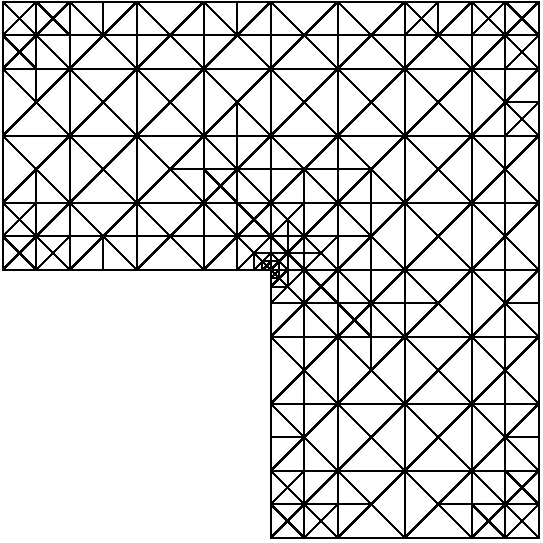
\includegraphics[width=.49\linewidth]{lshape_afem.eps}
  \includegraphics[width=.49\linewidth]{crackone_afem.eps}
  \caption{The left image corresponds to the L-shaped domain, the right corresponds to the cracked domain. Three methods are
  compared by plotting the approximation error $\uaenorm{\tilde U_k - U_K}_\O$ against the number of vertices. The adaptive methods
  used D\"orfler marking $\theta = 1/2$.}
  \label{fig:afem}
\end{figure}

\section{Mixed finite element solution}
Prager and Synge' theorem provided us with the following upper bound:
\[
  \enorm{u - U_h}_{\O}^2  \leq \norm{\nabla U_h - \vsig}^2_{\O} \quad \text{ for } \vsig \in H(\div; \O) \text{ s.t. } \div \v{\sigma} + f = 0
\]
The equilibrated method constructs $\v{\zeta} \in \RT_p(\O)$ such that $-\v{\zeta}$ satisfies the equilibrium condition, and thus we find an
upper bound in terms of $\nabla U_h + \v{\zeta}$. As noted before, the best upper bound with $\vsig \in \RT_p(\O)$ is found by minimizing
$\norm{\nabla U_h - \vsig}^2_{\O}$ for all fluxes $\vsig$ that are in equilibrium. Since this method is too expensive for an estimator
calculation the alternative of solving local minimization problems was introduced. The mixed finite element method provides the $\vsig$ that 
globally minimizes this norm. It is therefore interesting to compare their performance.

The iFEM package ships with an implementation of the lowest order mixed finite element solution. In Figure~\ref{fig:effmixed} the results are given. One image plots the efficiency indices of the mixed and equilibrated estimator
for the above domains. In every case the mixed estimator has a higher efficiency index as one would expect. 
More surprising is the behaviour for the unit square problems. The efficiency coefficients of the equilibrated estimator
seem to  converge to the efficiency coefficient of the mixed estimator. This suggests that the penalty of applying
local instead of global minimization decreases for large triangulations. For the L-shape and crack domain we have different behaviour,
both the efficiency indices seem to decreases for large triangulations. 
\begin{figure}
  \centering
  \includegraphics[width=.8\linewidth]{efficiency_mixed.eps}
  \caption{
    Compares the efficiency index of the equilibrated estimator (dashed lines) against the mixed estimator (solid lines), for
  four different domains indicated by color and marker styles.}
  \label{fig:effmixed}
\end{figure}

The mixed estimator provides a local error estimator by restricting the norm to an element, i.e. $\uanorm{\nabla U_h - \vsig}^2_K$. We
can use this estimator to drive AFEM. Figure~\ref{fig:afemmixed} compares this method to the others for the cracked domain with D\"orfler marking $\theta = 3/10$. 
As before all of these methods produce discrete solutions of the same approximation quality. 
\begin{figure}
  \centering
  \includegraphics[width=.8\linewidth]{afem_mixed.eps}
  \caption{
    Approximation quality of various (A)FEM solutions for the cracked domain. The adaptive solutions are found using $\theta = 3/10$.
  }
  \label{fig:afemmixed}
\end{figure}
\end{document}
